\chapter{Analisis}
\label{chap:analisis}

Bab ini membahas tentang analisis kebutuhan Sharif Judge yang diperlukan oleh Teknik Informatika dan solusi yang ditawarkan untuk memenuhi kebutuhan tersebut. Kebutuhan-kebutuhan tersebut didapat dari daftar isu repositori Sharif Judge di \textit{GitHub} dan dari para dosen pengguna Sharif Judge. Hasil dari analisis kebutuhan tersebut dicatat ke dalam \textit{Google Sheets} dan didiskusikan dengan dosen pembimbing. Selain analisis kebutuhan, pada bab ini juga akan dibahas analisis sistem kini pada perangkat lunak Sharif Judge.


\section{Analisis Kebutuhan Perangkat Lunak Sharif Judge}
\label{sec:analisis}
Analisis dilakukan dengan menganalisis setiap isu terbuka yang ada pada repositori di GitHub. Setiap isu di GitHub terdapat kode unik yang dimulai dengan tanda '\#' dan diikuti dengan angka. Kode unik tersebut menunjukan urutan isu yang dibuat oleh para pengguna GitHub. Dari analisa setiap isu yang ada, didapatkan beberapa pertanyaan dan usulan pengembangan. Beberapa isu yang memiliki usulan pengembangan akan dijadikan pertimbangan untuk mengembangkan Sharif Judge. \\

Analisis kebutuhan dari para dosen pengguna Sharif Judge dilakukan dalam bentuk wawancara secara langsung dan melalui email. Dosen-dosen yang telah diwawancarai antara lain:
\begin{enumerate}
	\item Husnul Hakim
	\item Claudio Franciscus
	\item Vania Natali
	\item Luciana Abednego
	\item Joanna Helga
\end{enumerate}
%Dari hasil wawancara didapatkan beberapa kebutuhan yang sama dari setiap dosen pengguna Sharif Judge. 

\begin{table}[H] %atau h saja untuk "kira kira di sini"
	\centering 
	\caption{\textit{Tabel Analisis Kebutuhan Sharif Judge}}
	\label{tab:kebutuhan}
	\resizebox{\textwidth}{!}{%
	\begin{tabular}{|l|l|l|l|l|l|}
		\toprule
		No & Deskripsi & Sumber & \thead{\textit{Issue Number /} \\ Nama Mata Kuliah} & \thead{Pembuat \textit{Issue} \\ Nama Dosen} & Status\\
		
		\midrule
		1 & Security with PHP & GitHub & \#61 & kathiedart & Diimplemntasi\\ \hline
		2 & Securing Assignment  & GitHub & \#55 & wojcik13 & Tidak diimplementasi\\ \hline
		3 & New Function & GitHub & \#53 & wojcik13 & Tidak diimplementasi\\ \hline
		4 & Solved Problem Indicator & GitHub & \#46 & atiabjobayer & Tidak diimplementasi\\ \hline
		5 & Some Problem \& Sugestion & GitHub & \#45 & atiabjobayer & Tidak diimplementasi\\ \hline
		6 & \makecell[l]{Queue failed to process if \\ submission take too long to \\ complete?}  & GitHub & \#32 & truongan & Diimplemntasi\\ \hline
		
		7 & Compilation Error on all language & GitHub & \#34 & Eririn07 & Tidak diimplementasi\\ \hline
		8 & \makecell[l]{Membatasi soal (deskripsi dan PDF) \\ hanya bisa diakses saat assignment \\ "open" dan setelah waktu mulai} & Dosen & ASD & Husnul Hakim & Diimplementasi\\ \hline
		
		9 & \makecell[l]{Menguji kemiripan kode antar \\ mahasiswa (Contek)} & Dosen & ASD & Husnul Hakim & Tidak diimplementasi\\ \hline
		10 & \makecell[l]{1 Akun hanya dapat login 1 waktu \\ (Jika suatu akun sedang login, tidak \\ ada lagi yang bisa login akun tersebut)} & Dosen & ASD & Husnul Hakim & Diimplementasi\\ \hline
		11 & \makecell[l]{Membatasi soal (deskripsi dan PDF) \\ hanya bisa diakses saat assignment \\ "open" dan setelah waktu mulai} & Dosen & ASD & Vania Natali & Diimplementasi\\ \hline
		12 & \makecell[l]{Sharif Judge tidak dapat menerima \\ file dengan ekstensi *.txt \\ untuk Pre-Test} & Dosen & ASD & Vania Natali & Diimplementasi\\ \hline
		13 & \makecell[l]{Membatasi soal (deskripsi dan PDF) \\ hanya bisa diakses saat assignment \\ "open" dan setelah waktu mulai} & Dosen & DAA & Luciana Abednego & Diimplementasi\\ \hline
		14 & \makecell[l]{Sharif Judge tidak dapat menerima \\ file dengan ekstensi *.txt \\ untuk Pre-Test} & Dosen & DAA & Luciana Abednego & Diimplementasi\\ \hline
		15 & \makecell[l]{Perlu ditambah petunjuk penamaan \\ file input \& output yg langsung \\ bisa dilihat ketika hendak upload} & Dosen & DAA & Luciana Abednego & Tidak diimplementasi\\ \hline
		16 & \makecell[l]{Membatasi soal (deskripsi dan PDF) \\ hanya bisa diakses saat assignment \\ "open" dan setelah waktu mulai} & Dosen & DAA & Joanna Helga & Diimplementasi\\ \hline
		17 & \makecell[l]{Register peserta yg mode batch, \\ Sharif Judge tidak minta nama \\ orangnya (lebih baik ada nama orangnya)} & Dosen & DAA & Joanna Helga & Diimplementasi\\ \hline
		18 & \makecell[l]{Nama peserta seharusnya tidak \\ bisa diganti (Bisa menjadi \\ "mainan" dan tindak kecurangan \\ karena dapat memberikan hint)} & Dosen & DAA & Joanna Helga & Diimplementasi\\ \hline
		19 & \makecell[l]{Ingin memiliki fungsi dimana \\ Assignment tidak memiliki batasan \\ waktu (arsip soal tahun \\ lalu dapat dikerjakan kapan saja)} & Dosen & DAA & Joanna Helga & Diimplementasi\\ \hline
		20 & \makecell[l]{Ingin memiliki scoreboard global \\ untuk semua assignment.} & Dosen & DAA & Joanna Helga & Diimplementasi\\ \hline
		21 & \makecell[l]{Membatasi soal (deskripsi dan PDF) \\ hanya bisa diakses saat assignment \\ "open" dan setelah waktu mulai} & Dosen & ASD \& DAA & Claudio Fransiscus & Diimplementasi\\ \hline
		22 & \makecell[l]{Sharif Judge tidak dapat menerima \\ file dengan ekstensi *.txt \\ untuk Pre-Test} & Dosen & ASD \& DAA & Claudio Fransiscus & Diimplementasi\\ \hline
		23 & \makecell[l]{UI masih merepotkan} & Dosen & ASD \& DAA & Claudio Fransiscus & Tidak diimplementasi\\ \hline
		24 & \makecell[l]{UI ada yang tidak berguna \\ (yang lebih banyak digunakan \\ assignment, submit, scoreboard, \\ dan hasil submit} & Dosen & ASD \& DAA & Claudio Fransiscus & Tidak diimplementasi\\

		\bottomrule
		
	\end{tabular}}
\end{table}

\begin{table}[H] %atau h saja untuk "kira kira di sini"
	\centering 
	%\caption{\textit{Kebutuhan Sharif Judge}}
	\label{tab:kebutuhan2}
	\resizebox{\textwidth}{!}{%
		\begin{tabular}{|l|l|l|l|l|l|}
			\hline
			25 & \makecell[l]{Ingin memiliki fungsi reminder. \\ Banyak mahasiswa lupa mengerjakan \\ tugas dan tidak bisa mengumpulkan. \\ Fungsi reminder akan mengirimkan \\ reminder ke email mahasiswa} & Dosen & ASD \& DAA & Claudio Fransiscus & Tidak diimplementasi\\ \hline
			26 & \makecell[l]{Membatasi soal (deskripsi dan PDF) \\ hanya bisa diakses saat assignment \\ "open" dan setelah waktu mulai} & Dosen & ASD \& DAA & Pascal Alfadian & Diimplementasi\\ \hline
			27 & \makecell[l]{Integrasi login ke RADIUS \\ (password sama dengan login Windows)} & Dosen & AIF401 & Pascal Alfadian & Diimplementasi\\ \hline
			28 & \makecell[l]{Mengumpulkan file TXT} & Dosen & AIF401 & Pascal Alfadian & Diimplementasi\\ \hline
			29 & \makecell[l]{Mengumpulkan file JAR (java multi kelas)} & Dosen & AIF401 & Pascal Alfadian & Diimplementasi\\ \hline
			30 & Branding Teknik Informatika & Dosen & AIF401 & Pascal Alfadian & Diimplementasi\\ \hline
	\end{tabular}}
\end{table}

Pada tabel diatas teradapat beberapa kolom, yaitu:
\begin{itemize}
	\item Deskripsi \\
	Jika sumber kebutuhan berasal dari GitHub, maka pada kolom deskripsi akan ditulis judul dari isu yang ada pada repositori. Jika sumber kebutuhan berasal dari dosen, maka deskripsi kebutuhan langsung ditulis pada kolom tersebut.
	\item Sumber \\
	Kolom sumber berisikan sumber dari kebutuhan pengembangan Sharif Judge yaitu GitHub atau Dosen.
	\item Issue Number / Nama Mata Kuliah \\
	Jika sumber kebutuhan berasal dari GitHub, maka pada kolom ini akan ditulis \hyperref[sec:analisis]{kode unik} yang ada pada setiap isu. Jika sumber kebutuhan berasal dari dosen, maka pada kolom ini akan ditulis mata kuliah yang diajar oleh dosen tersebut.
	\item Pembuat Issue / Nama Dosen \\
	Jika sumber kebutuhan berasal dari GitHub, maka pada kolom ini akan ditulis username pembuat isu tersebut. Jika sumber kebutuhan berasal dari dosen, maka pada kolom ini akan ditulis nama dosen yang memberikan daftar kebutuhan.
	\item Status \\
	Kolom Status berisikan status dari kebutuhan tersebut apakah akan diimplementasi atau tidak diimplementasi.
\end{itemize}

%Pada tabel diatas terdapat kolom Deskirpsi, Sumber, Issue Number / Nama Mata Kuliah, Pembuat Issue / Nama Dosen dan Status. Kolom Deskripsi berisikan deskripsi kebutuhan yang disebutkan oleh para dosen, namun jika sumber kebutuhan berasal dari GitHub maka akan berisikan judul isu. Kolom Sumber berisikan sumber kebutuhan yaitu GitHub atau Dosen. Kolom Issue Number / Nama Mata Kuliah berisikan 

\subsection{\textit{Security with PHP}}
Isu dengan kode unik \#61 dibuat oleh pengguna \textit{GitHub} dengan username \textit{danwdart} pada tanggal 6 April 2017. Pada isu tersebut dikatakan bahwa seseorang pengguna Sharif Judge dapat mengubah parameter PHP \textit{shell\_exec(rm ...)} yang mengakibatkan pengeksekusian kode bisa dilakukan secara sewenang-wenang. Untuk menghindari hal diatas, username \textit{danwdart} menyarankan untuk mengganti perintah PHP \textit{shell\_exec(rm ...)} dengan method lain.

Pada skripsi ini, isu diatas akan diperbaiki. Solusi yang ditawarkan adalah mengganti penggunaan PHP \textit{shell\_exec(rm ...)} dengan method lain.  Perintah \textit{shell\_exec("rm ...")} memiliki fungsi untuk menghapus sebuah file. Perintah tersebut dapat diganti menggunakan method \textit{unlink()} yang memiliki fungsi sama yaitu menghapus sebuah file.
%Hal tersebut dapat dicegah dengan cara mengubah perintah shell\_exec("rm ...") dengan method \textit{unlink()}.

\subsection{Securing Assignment}
Isu dengan kode unik \#55 dibuat oleh pengguna \textit{GitHub} dengan username \textit{wojcik13} pada tanggal 23 Oktober 2016. Username \textit{wojcik13} menanyakan apakah ada pilihan pada Sharif Judge untuk mengamankan assignment dengan password.

Pada skripsi ini, isu diatas tidak diperbaiki. Isu diatas merupakan sebuah pertanyaan fitur pada Sharif Judge untuk mengamankan assignment dengan menggunakan password. Oleh karena isu tersebut merupakan sebuah pertanyaan, maka pada skripsi ini isu diatas tidak diperbaiki.

\subsection{New Function}
Isu dengan kode unik \#53 dibuat oleh pengguna \textit{GitHub} dengan username \textit{wojcik13} pada tanggal 2 Oktober 2016. Username \textit{wojcik13} menanyakan apakah ada fungsi pada Sharif Judge seperti menghentikan scoreboard dan fungsi mengatur sesi. 

Pada skripsi ini, isu diatas tidak diperbaiki. Isu diatas merupakan sebuah pertanyaan fitur pada Sharif Judge untuk menghentikan scoreboard dan mengatur sesi. Oleh karena isu tersebut merupakan sebuah pertanyaan, maka pada skripsi ini isu diatas tidak diperbaiki.

\subsection{Solve Problem Indicator}
Isu dengan kode unik \#46 dibuat oleh pengguna \textit{GitHub} dengan username \textit{atiabjobayer} pada tanggal 16 April 2016. Username \textit{atiabjobayer} mengatakan bahwa para pengguna Sharif Judge tidak dapat melihat masalah yang telah diselesaikan.

Pada skripsi ini, isu diatas tidak diperbaiki. Pada isu diatas, username \textit{atiabjobayer} kurang spesifik dalam menjelaskan kebutuhannya.
Oleh karena isu tersebut kurang spesifik, maka pada skripsi ini isu diatas tidak diperbaiki.

\subsection{Some Problem \& Sugestion}
Isu dengan kode unik \#45 dibuat oleh pengguna \textit{GitHub} dengan username \textit{atiabjobayer} pada tanggal 16 April 2016. Username \textit{atiabjobayer} mengatakan bahwa ada beberapa persoalan yang ada pada perangkat lunak Sharif Judge. Beberapa masalah tersebut yaitu:
	\begin{enumerate}
		\item Beberapa kontes besar pemrograman diadakan dengan metode ACM ICPC namun Sharif Judge tidak mendukung sistem penilaian ICPC.
		\item Pengguna dapat melihat deskripsi masalah sebelum kontes dimulai. Hal ini dapat membahayakan keamanan kontes pemrograman.
		\item Tampilan yang digunakan pada Sharif Judge tidak responsif. Pengguna tidak dapat melihat pada \textit{device} kecil/
		\item Seharusnya ada Sistem Klarifikasi. Fitur ini harus ada pada \textit{online judge}.
		\item Pengguna tidak dapat mengumpulkan kode mereka dari text-editor.
	\end{enumerate}

Pada skripsi ini, isu diatas tidak diperbaiki. Isu diatas memiliki cakupan persoalan yang terlalu luas. Username \textit{atiabjobayer}. Oleh karena isu tersebut memiliki persoalan yang terlalu luas, maka pada skripsi ini isu diatas tidak diperbaiki.
	
\subsection{\textit{Queue failed to process if submission take too long to complete?}}
Isu dengan kode unik \#32 dibuat oleh pengguna \textit{GitHub} dengan username \textit{truongan}. Pada isu tersebut dikatakan bahwa assignment yang memiliki masalah dengan test case besar akan menyebabkan \textit{submission status} menjadi \textit{pending}. User \textit{truongan} memperkirakan hal diatas terjadi dikarenakan \textit{database connection times out}. 

Pada skripsi ini, isu diatas akan diperbaiki. Solusi yang ditawarkan untuk mengatasi hal diatas adalah menambahakan \textit{method reconnect database}. \textit{Method reconnect database} akan menghubungkan kembali database ketika terjadi kasus seperti diatas.
% Untuk mengatasi masalah tersebut diperlukan method reconnect database pada file \textit{Queueprocess.php}.

\subsection{Compilation Error on All Language}
Isu dengan kode unik \#34 dibuat oleh pengguna \textit{GitHub} dengan username \textit{Eririn07}. Username \textit{Eririn07} mencoba untuk menilai sebuah kode dan mendapatkan beberapa error. Kode error yang muncul ketika menilai kode dengan bahasa \textit{Java adalah Java HotSpot(TM) 64-Bit Server VM warning: INFO: os::commit\_memory(0x00007f9cfd000000, 2555904, 1) failed; error='Permission denied' (errno=13)} dan Kode error \textit{File Not Found} muncul ketika menilai kode dengan bahasa C. Username \textit{Eririn07} menanyakan bagaimana mengatasi masalah diatas.

Pada skripsi ini, isu diatas tidak diperbaiki. Isu diatas merupakan sebuah pertanyaan untuk mengatasi kode error yang muncul. Oleh karena isu tersebut merupakan sebuah pertanyaan, maka pada skripsi ini isu diatas tidak diperbaiki.

\subsection{Membatasi soal (deskripsi \& PDF) hanya bisa diakses saat assignment "open" dan setelah waktu mulai}
\label{subsec:membatasisoal}
Kebutuhan ini merupakan salah satu kebutuhan yang paling banyak disebut oleh para dosen pengguna Sharif Judge. Perangkat lunak Sharif Judge terkini masih belum dapat memenuhi kebutuhan diatas. Para peserta dapat mengunduh deskripsi soal \& PDF sebelum waktu assignment dimulai. Untuk menangani hal tersebut para dosen harus mengunggah file PDF tepat pada saat assignment dimulai. 

Pada skripsi ini, kebutuhan diatas akan diimplementasi. Solusi yang ditawarkan untuk memenuhi kebutuhan diatas yaitu membatasi soal agar dapat diunduh pada saat assignment "open" dan setelah waktu mulai. Jika ada peserta yang mencoba untuk mengunduh soal (deskripsi \& PDF) pada saat assignment belum dimulai, maka akan muncul pesan error \textit{"Selected \textit{assignment"} has not started.} Deskripsi \& PDF hanya dapat diunduh tepat setelah waktu assignment dimulai.

\subsection{Menguji kemiripan kode antar mahasiswa}
Perangkat lunak Sharif Judge terkini sudah memiliki fitur untuk menguji kemiripan kode antar peserta dengan menggunakan Moss (\textit{Measure Of Software Similarity}). Moss adalah sistem otomatis untuk mendeteksi kemiripan program. Aplikasi Moss telah berkembang dari tahun 1994 hingga sekarang. Algoritma yang digunakan pada aplikasi Moss sangat efektif dibandingkan algoritma deteksi kecurangan lainnya~\cite{aiken:10:moss}. 

Pada skripsi ini, kebutuhan diatas tidak diimplementasi karena aplikasi Moss sedang tidak dapat digunakan. Hal tersebut terjadi karena aplikasi Moss membutuhkan port 7690, namun port tersebut diblok oleh UNPAR.

\subsection{Satu Akun hanya dapat login satu waktu}
Para peserta Sharif Judge dapat login menggunakan akunnya di beberapa komputer. Peserta yang mengetahui user dan password peserta lain dapat dengan mudah login ke Sharif Judge. Hal tersebut sering dijadikan celah bagi beberapa peserta untuk melakukan tindak kecurangan. Peserta yang sudah login menggunakan akun peserta lainnya, dapat melihat dan menyalin kode yang telah dikumpulkan ke Sharif Judge. Tindak kecurangan ini sering terjadi pada saat kuis maupun ujian. Bapak Husnul Hakim menginginkan perangkat lunak Sharif Judge dimana akun para peserta hanya dapat login satu waktu. Jika sebuah akun telah login di satu komputer, maka akun tersebut tidak dapat login di komputer lainnya. Diharapkan dengan adanya fitur tersebut dapat menekan jumlah tindak kecurangan yang terjadi. 

Pada skripsi ini, kebutuhan diatas tidak diimplementasi. Jika fitur diatas diimplementasi, maka ditakutkan akan merepotkan admin. Para admin harus membuka akun pengguna setiap kali ada akun yang terkunci pada sebuah komputer. Sebagai gantinya, penulis menawarkan sebuah solusi. Solusi yang ditawarkan untuk mengurangi tingkat kecurangan seperti diatas yaitu membuat halaman baru yang berisikan \textit{logs} username yang berhasil login ke Sharif Judge. Halaman logs tersebut akan mencatat username yang login menggunakan ip berbeda dalam waktu dibawah 24 jam. Dengan adanya halaman Logs ini, para dosen dapat memantau username yang login pada dua tempat berbeda.	

\subsection{Membatasi soal (deskripsi \& PDF) hanya bisa diakses saat assignment "open" dan setelah waktu mulai}
Kebutuhan ini telah dibahas pada sub bab sebelumnya. Lihat sub bab \hyperref[subsec:membatasisoal]{3.1.8} untuk status dari kebutuhan ini.

\subsection{Mengumpulkan file dengan format TXT}
\label{subsec:filetxt}
Pengumpulan file dengan format TXT dibutuhkan untuk \textit{Pre-test}. Perangkat lunak Sharif Judge yang sekarang hanya dapat menerima file C, C++, Java, Python 2, Python 3, Zip, dan PDF. Para peserta yang ingin mengumupulkan jawaban \textit{Pre-test}, harus terlebih dahulu mengubah ekstensi file menjadi Java atau mengompres file ke dalam Zip. 

Pada skripsi ini, kebutuhan diatas akan diimplementasi. Solusi yang ditawarkan untuk kebutuhan diatas yaitu menambahkan file dengan format TXT agar dapat dikumpul ke Sharif Judge. Assignment yang digunakan merupakan assignmnent yang bersifat "Upload Only". Dosen dapat menambahkan format TXT pada bagian "Allowed Language" sehingga para peserta dapat mengumpulkan jawaban \textit{Pre-test} menggunakan file dengan ekstensi TXT.

\subsection{Membatasi soal (deskripsi \& PDF) hanya bisa diakses saat assignment "open" dan setelah waktu mulai}
Kebutuhan ini telah dibahas pada sub bab sebelumnya. Lihat sub bab \hyperref[subsec:membatasisoal]{3.1.8} untuk status dari kebutuhan ini.

\subsection{Mengumpulkan file dengan format TXT}
Kebutuhan ini telah dibahas pada sub bab sebelumnya. Lihat sub bab \hyperref[subsec:filetxt]{3.1.12} untuk status dari kebutuhan ini.

\subsection{Perlu ditambah petunjuk penamaan file input dan output}
Dalam membuat sebuah assignment pada perangkat lunak Sharif Judge terdapat file test case yang harus disertakan. File test case yang disertakan memiliki beberapa ketentuan. Beberapa ketentuan tersebut seperti struktur direktori dan penamaan dalam file test case. 

Pada skripsi ini, kebutuhan diatas tidak diimplementasi. Pada halaman add assignment telah disediakan link menuju dokumentasi Sharif Judge di \textit{GitHub} yang menjelaskan ketentuan dalam menyertakan file test case. Ketentuan tersebut harus terpenuhi agar sebuah assignment dapat berjalan dengan baik. Oleh sebab itu, kebutuhan ini tidak diimplementasi.

\subsection{Membatasi soal (deskripsi \& PDF) hanya bisa diakses saat assignment "open" dan setelah waktu mulai}
Kebutuhan ini telah dibahas pada sub bab sebelumnya. Lihat sub bab \hyperref[subsec:membatasisoal]{3.1.8} untuk status dari kebutuhan ini.

\subsection{Pendaftaran peserta disertai dengan \textit{Display Name}}
Pendaftaran peserta ke dalam Sharif Judge terkini tidak disertai dengan \textit{Display Name}. Perangkat lunak Sharif Judge membutuhkan empat buah parameter yang dipisah menggunakan spasi untuk mendaftarkan peserta. Parameter tersebut antara lain, username, email, password dan role. Contoh penggunaannya seperti "i14085 i14085@unpar.ac.id random85 student" yang artinya peserta didaftarkan menggunakan username i14085, email i14085@unpar.ac.id, password random85 dan role sebagai student. Setiap peserta yang berhasil didaftarkan masih belum memiliki \textit{Display Name}. Para peserta harus memasukan \textit{Display Name} masing-masing secara manual. 

Pada skripsi ini, kebutuhan diatas akan diimplementasi. Solusi yang ditawarkan untuk memenuhi kebutuhan diatas yaitu menambahkan parameter \textit{Display Name} pada saat pendaftaran peserta. Parameter yang digunakan akan menjadi lima buah paramater dan dipisah menggunakan tanda koma. Parameter tersebut antara lain, username, email, display name, password, dan role. Contoh penggunaan parameter diatas seperti "i14085,i14085@unpar.ac.id,Budi Simon,random85,student" yang artinya peserta didaftarkan menggunakan username i14085, email i14085@unpar.ac.id, display name Budi Simon, password random85 dan role sebagai student. Dengan pengimplementasian fitur ini, setiap peserta yang didaftarkan akan langsung memiliki Display Name masing-masing.

\subsection{Nama pengguna Sharif Judge seharusnya tidak bisa diubah}
\textit{Display Name} pada perangkat lunak Sharif Judge berfungsi sebagai nama peserta. Selain itu, nama peserta akan muncul pada halaman Scoreboard sebuah assignment yang dapat dilihat oleh seluruh peserta. Sharif Judge yang terkini mengijinkan para peserta untuk mengubah \textit{Display Name} pada halaman Profile. Hal tersebut dapat dijadikan sebuah "mainan" dan tindakan kecurangan karena dapat memberikan \textit{hint} untuk peserta lain. Oleh karena itu, Ibu Joanna Helga menginginkan nama peserta yang terdaftar pada Sharif Judge tidak dapat diubah. 

Pada skripsi ini, kebutuhan diatas akan diimplementasi. Solusi yang ditawarkan untuk memenuhi kebutuhan diatas yaitu menambahkan sebuah fitur dimana fitur tersebut dapat mengunci \textit{Display Name} peserta Sharif Judge. Fitur ini akan diletakan pada halaman Settings yang dapat diatur oleh admin. Jika admin mengaktifkan fitur tersebut, maka \textit{input text Display Name} pada halaman Profile menjadi nonaktif sehingga para peserta tidak dapat mengubah \textit{Display Name}. Sebaliknya jika admin menonaktifkan fitur tersebut, maka \textit{input text Display Name} pada halaman Profile akan kembali aktif.

\subsection{Sharif Judge diharapkan memiliki fungsi dimana assignment dapat dikumpulkan tanpa adanya batasan waktu}
Pada masa Pra UTS dan Pra UAS biasanya para dosen akan memberikan assignment sebagai bahan pembelajaran. Arsip-arsip soal ujian dan latihan tahun lalu akan dijadikan sebuah assignment yang dapat dikerjakan oleh para peserta. Assignment tersebut memiliki waktu pengumpulan yang cenderung lama. Ibu Joanna Helga menginginkan sebuah fitur dimana Sharif Judge dapat mengatur assignment tertentu menjadi tidak memiliki batasan waktu dan dapat dikumpulkan kapan saja. 

Pada skripsi ini, kebutuhan diatas akan diimplementasi. Solusi yang ditawarkan untuk memenuhi kebutuhan diatas yaitu membuat sebuah fitur tambahan pada assignment. Fitur tersebut akan membuat batas waktu pengumpulan menjadi tanggal 18 Januari 2038. Assignment yang mengaktifkan fitur tidak akan muncul pada kalendar yang terdapat di halaman Dashboard.

\subsection{Sharif Judge diharapkan memiliki Scoreboard global untuk semua assignment}
Sharif Judge terkini memiliki halaman Scoreboard yang berfungsi menampilkan seluruh nilai akhir para peserta dari sebuah assignment. Pada halaman Socreboard juga menampilkan nilai dari setiap problem yang ada pada sebuah assignment. Nilai yang muncul pada halaman ini adalah nilai para peserta yang telah mengumpulkan jawabannya. Nilai yang muncul tersebut akan diurutkan mulai dari yang tertinggi hingga terendah. Para dosen menginginkan sebuah Scoreboard global untuk semua assignment. Scoreboard global tersebut akan menampilkan berapa problem yang telah dikerjakan para peserta diseluruh assignment yang ada. 

Pada skripsi ini, kebutuhan diatas akan diimplementasi. Solusi yang ditawarkan untuk memenuhi kebutuhan diatas yaitu membuat halaman baru yang diberi nama Hall of Fame. Halaman Hall of Fame akan menampilkan berapa problem yang telah dikerjakan oleh para peserta diseluruh assignment yang ada. Nama peserta yang muncul pada halaman ini diurutkan sesuai dengan banyaknya problem yang berhasil diselsaikan oleh para peserta.

\subsection{Membatasi soal (deskripsi \& PDF) hanya bisa diakses saat assignment "open" dan setelah waktu mulai}
Kebutuhan ini telah dibahas pada sub bab sebelumnya. Lihat sub bab \hyperref[subsec:membatasisoal]{3.1.8} untuk status dari kebutuhan ini.

\subsection{Mengumpulkan file dengan format TXT}
Kebutuhan ini telah dibahas pada sub bab sebelumnya. Lihat sub bab \hyperref[subsec:filetxt]{3.1.12} untuk status dari kebutuhan ini.

\subsection{UI masih merepotkan}

\subsection{UI ada yang tidak berguna}

\subsection{Sharif Judge diharapkan memiliki fungsi reminder}
Setiap assignment pada perangkat lunak Sharif Judge memiliki batas pengumpulan. Jika assignment telah melewati batas pengumpulan maka para peserta tidak dapat mengumpulkan tugasnya. Banyak peserta sering kali lupa untuk mengerjakan assignment dan pada akhirnya melewati batas pengumpulan. Bapak Claudio Fransiscus menginginkan perangkat lunak Sharif Judge yang memiliki fitur reminder. Fitur reminder akan mengirimkan email ke setiap peserta yang berisikan peringatan bahwa ada assignment yang harus diselsaikan. 

Pada skripsi ini, kebutuhan diatas tidak diimplementasi. Kebutuhan diatas belum dapat diimplementasi karena masih belum ada sistem \textit{scheduler}. Selain itu, bobot pekerjaan diperkirakan akan membutuhkan waktu lebih dari 1 semester.

\subsection{Membatasi soal (deskripsi \& PDF) hanya bisa diakses saat assignment "open" dan setelah waktu mulai}
Kebutuhan ini telah dibahas pada sub bab sebelumnya. Lihat sub bab \hyperref[subsec:membatasisoal]{3.1.8} untuk status dari kebutuhan ini.

\subsection{Integrasi login ke RADIUS}
RADIUS (\textit{Remote Authentication Dial In User Service}) merupakan protokol jaringan klien dan server. Klien mengirimkan informasi pengguna ke server RADIUS yang ditunjuk dan akan bertindak berdasarkan respons yang dikembalikan. Server RADIUS akan menerima permintaan koneksi pengguna, mengautentikasi pengguna dan kemudian mengembalikan informasi konfigurasi yang diperlukan agar klien dapat memberikan layanan kepada pengguna. Server RADIUS dapat bertindak sebagai klien proxy ke server RADIUS lain atau server autentikasi jenis lainnya \footnote{Cisco, "How Does RADIUS Work?" How Does RADIUS Work? - Cisco. \textit{https://www.cisco.com/c/en/us/support/docs/security-vpn/remote-authentication-dial-user-service-radius/12433-32.html} (diakses 22 Februari 2018)}. %footnote .
Lab FTIS UNPAR memiliki server RADIUS yang dapat memverifikasi ID mahasiswa terhadap kata sandinya. Server RADIUS juga berguna untuk autentikasi ID mahasiswa agar menggunakan komputer di Lab FTIS UNPAR.

Pada skripsi ini, kebutuhan diatas akan diimplementasi. Solusi yang ditawarkan untuk memenuhi kebutuhan diatas yaitu mengintegrasikan lagin server RADIUS pada perangkat lunak Sharif Judge. Dengan pengimplementasian integrasi login RADIUS pada Sharif Judge, para peserta dapat login ke Sharif Judge menggunakan akun yang terdapat pada server RADIUS. 

\subsection{Mengumpulkan file dengan format TXT}
Kebutuhan ini telah dibahas pada sub bab sebelumnya. Lihat sub bab \hyperref[subsec:filetxt]{3.1.12} untuk status dari kebutuhan ini.

\subsection{Mengumpulkan file JAR (java multi kelas)}
JAR (Java ARchive) adalah format file platform-independen yang menggabungkan banyak file menjadi satu. File-file seperti kelas, gambar dan suara dapat digabungkan dalam file JAR. ==On Progress==

\subsection{Branding Teknik Informatika}
Branding Teknik Informatika akan dilakukan dengan cara mengubah logo dan ikon Sharif Judge menjadi logo Teknik Informatika. Selain mengubah logo dan ikon, perubahan juga akan dilakukan terhadap nama perangkat lunak menjadi SharIF Judge dan link dokumentasi yang ada pada perangkat lunak Sharif Judge. Hal diatas dapat dilakukan karena Sharif Judge sendiri menggunakan lisensi GPL versi 3. GPL merupakan kepanjangan dari General Public License yang memberikan beberapa kebebasan pada setiap penggunanya~\cite{brett:10:moss}.
Kebebasan tersebut antara lain:
	\begin{itemize}
		\item Kebebasan untuk menggunakan perangkat lunak dengan tujuan apapun \\
		\item Kebebasan untuk mengubah perangkat lunak sesuai dengan kebutuhan \\
		\item Kebebasan untuk membagikan perangkat lunak kepada teman dan kerabat \\
		\item Kebebasan untuk membagikan perubahan yang telah dilakukan
	\end{itemize}
Pada skripsi ini, kebutuhan diatas akan diimplementasi. Beberapa logo yang akan digunakan seperti:

\begin{figure}[H]
	\centering  
	
\includegraphics[scale=1]{logosmall}  
	\caption[Logo dan Ikon]{Logo dan Ikon} 
	\label{fig:logosmall} 
\end{figure} 

\begin{figure}[H]
	\centering  
	
\includegraphics[scale=1]{banner}  
	\caption[\textit{Banner} SharIF Judge]{\textit{Banner} SharIF Judge} 
	\label{fig:banner} 
\end{figure} 

\pagebreak

Berikut beberapa tampilan SharIF Judge yang baru.
\begin{figure}[H]
	\centering  
	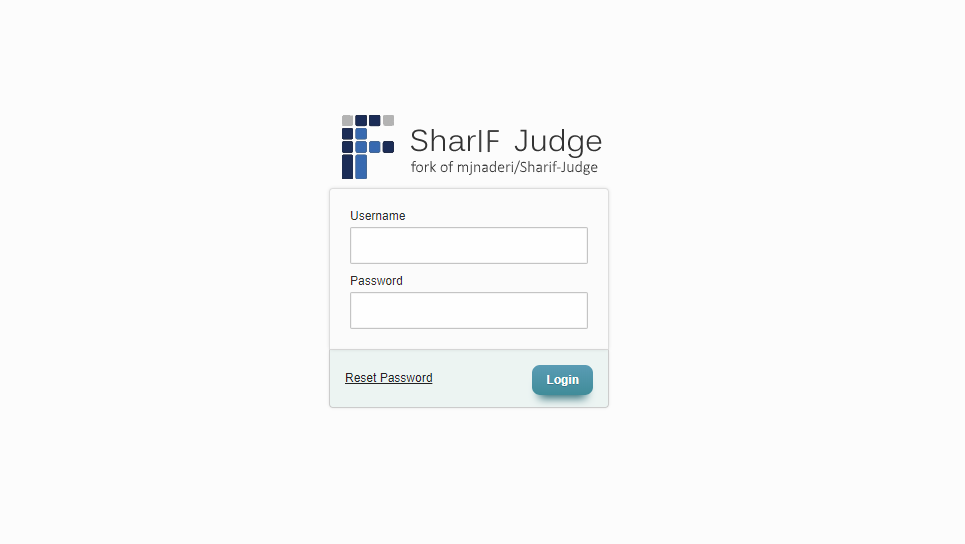
\includegraphics[scale=0.5]{login}  
	\caption[Halaman Login SharIF Judge]{Halaman Login SharIF Judge} 
	\label{fig:login} 
\end{figure}

\begin{figure}[H]
	\centering  
	
\includegraphics[scale=1]{ikon}  
	\caption[Ikon SharIF Judge pada Title Bar]{Ikon SharIF Judge pada Title Bar} 
	\label{fig:ikon} 
\end{figure} 

\begin{figure}[H]
	\centering  
	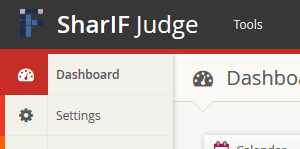
\includegraphics[scale=1]{logo}  
	\caption[Logo SharIF Judge pada Top Bar]{Logo SharIF Judge pada Top Bar} 
	\label{fig:logo} 
\end{figure} 

\pagebreak

\section{Analisis Sistem Kini}

Seperti yang telah dibahas pada \hyperref[sec:sharifjudge]{Bab 2.2}, Sharif Judge menggunakan framework Codeigniter. Framework ini menerapkan prinsip Model-View-Controller (M-V-C). Model-View-Controller merupakan metode untuk membuat sebuah aplikasi dengan memisahkan data (Model) dari tampilan (View) dan cara memprosesnya (Controller). Pada perangkat lunak Sharif Judge model, view dan controller terdapat pada folder Application serta dipisahkan ke dalam masing-masing folder.  

\subsection{Model}
Di dalam folder {Model}, terdapat beberapa file model yang berisikan fungsi-fungsi untuk membantu pengguna mengambil, menyimpan, dan memperbarui informasi pada database.

\subsubsection{Assignment\_Model.php}
Pada file Assignment\_Model.php terdapat beberapa fungsi yaitu:
\begin{itemize}
	\item add\_assignment: menambahkan assignment baru ke dalam database atau mengedit assignment yang ada
	\item delete\_assignment: menghapus assignment 
	\item all\_assignments: menampilkan semua daftar assignment dan informasinya
	\item new\_assignment\_id: mengembalikan nilai int terkecil yang dapat digunakan sebagai id untuk assignment baru
	\item all\_problems: mengembalikan array yang berisi semua masalah dalam assignment yang diberikan
	\item problem\_info: mengembalikan baris database untuk masalah tertentu
	\item assignment\_info: mengembalikan baris database untuk assignment tertentu
	\item is\_participant: mengecek apakah pengguna terdaftar sebagai peserta pada assignment tertentu
	\item increase\_total\_submits: meningkatkan jumlah total submit sebanyak satu
	\item set\_moss\_time: mengedit "\textit{Moss Update Time}" untuk assingment tertentu
	\item get\_moss\_time: mengembalikan "\textit{Moss Update Time}" untuk assingment tertentu
	\item save\_problem\_description: menambahkan atau Memperbarui deskripsi masalah
	\item \_update\_coefficients: memperbarui koefisien yang terdapat pada assignment tertentu. Fungsi ini akan dipanggil oleh fungsi add\_assignment
\end{itemize}

\subsubsection{Notifications\_Model.php}
Pada file Notifications\_Model.php terdapat beberapa fungsi yaitu:
\begin{itemize}
	\item get\_all\_notifications: mengembalikan semua notifikasi
	\item get\_latest\_notifications: mengembalikan 10 notifikasi terkini
	\item add\_notification: menambahkan notifikasi baru
	\item update\_notification: mengedit notifikasi tertentu
	\item delete\_notification: menghapus notifikasi tertentu
	\item get\_notification: menampilkan notifikasi tertentu
	\item have\_new\_notification: mengecek apakah terdapat notifikasi setelah melewati waktu tertentu
\end{itemize}

\subsubsection{Queue\_Model.php}
Pada file Queue\_Model.php terdapat beberapa fungsi yaitu:
\begin{itemize}
	\item in\_queue: mengecek apakah sebuah submission telah berada dalam antrian
	\item get\_queue: mengembalikan semua antrian submission
	\item empty\_queue: mengosongkan antrian
	\item add\_to\_queue: memasukan submission ke dalam antrian
	\item rejudge: menambahkan submission ke dalam antrian untuk di-\textit{rejudge}
	\item rejudge\_single: menambahkan submission tunggal ke dalam antrian untuk di-\textit{rejudge}
	\item get\_first\_item: mengembalikan item pertama dari antrian
	\item remove\_item: menghapus item tertentu dari antrian
	\item save\_judge\_result\_in\_db: menyimpan hasil dari \textit{judge} ke dalam database. Fungsi ini akan dipanggil oleh fungsi Queueprocess di Controller
\end{itemize}

\subsubsection{Scoreboard\_Model.php}
Pada file Scoreboard\_Model.php terdapat beberapa fungsi yaitu:
\begin{itemize}
	\item \_generate\_scoreboard: menghasilkan scoreboard dari Final Submissions untuk assignment tertentu. Fungsi ini akan dipanggil oleh update\_scoreboard
	\item update\_scoreboards: mengupdate \textit{cache} scoreboard dari semua assignment. Fungsi ini akan dipanggil setiap kali pengguna menghapus atau semua assignment pengguna dihapus.
	\item update\_scoreboard: mengupdate cache scoreboard dari semua assignment dan menyimpan kode html scoreboard ke dalam database. Fungsi ini dipanggil setelah judging/rejudging sebuah submission dan ketika beberapa settings diubah pada assignment tertentu. Setting tersebut terdiri dari Extra Time, Start Time, Finish Time, Coefficient's Rule dan Enable/Disable Scoreboard.
	\item get\_scoreboard: mengembalikan \textit{cache} scoreboard untuk assignment tertentu sebagai teks html
\end{itemize}

\subsubsection{Settings\_Model.php}
Pada file Settings\_Model.php terdapat beberapa fungsi yaitu:
\begin{itemize}
	\item get\_setting: mengembalikan pengaturan tertentu
	\item set\_setting: mengupdate pengaturan tertentu
	\item get\_all\_settings: menampilkan semua pengaturan
	\item set\_setting: mengupdate seluruh pengaturan
\end{itemize}

\subsubsection{Submit\_Model.php}
Pada file Submit\_Model.php terdapat beberapa fungsi yaitu:
\begin{itemize}
	\item get\_submission: mengembalikan baris tabel sebuah submission tertentu 
	\item get\_final\_submissions: mengembalikan baris tabel final submission para peserta dari sebuah submission tertentu
	\item get\_all\_submissions: mengembalikan baris tabel seluruh submission
	\item count\_final\_submissions: mengembalikan jumlah total final submission dari peserta tertentu
	\item count\_all\_submissions: mengembalikan jumlah total submission dari peserta tertentu
	\item set\_final\_submission: menentukan submission tertentu agar menjadi final submission
	\item add\_upload\_only: menambahkan hasil dari submit "Upload only" ke database
\end{itemize}

\subsubsection{User.php}
Pada file User.php terdapat beberapa fungsi yaitu:
\begin{itemize}
	\item select\_assignment: menetapkan assignment yang dipilih untuk username tertentu
	\item save\_widget\_positions: mengupdate posisi dari dashboard widget ke database
	\item get\_widget\_positions: mengembalikan posisi dashboard widget dari database
\end{itemize}

\subsubsection{User\_Model.php}
Pada file User\_Model.php terdapat beberapa fungsi yaitu:
\begin{itemize}
	\item have\_user: mengecek apakah pengguna dengan username yang diinput terdapat di database
	\item user\_id\_to\_username: mengubah user id menjadi username
	\item username\_to\_user\_id: mengubah username menjadi user id
	\item have\_email: mengecek apakah pengguna dengan email yang diberikan terdapat di database
	\item add\_user: menambahkan pengguna tunggal
	\item add\_users: menambahkan beberapa pengguna
	\item delete\_user: menghapus pengguna tertentu
	\item delete\_submissions: menghapus semua submission pengguna tertentu
	\item validate\_user: mengecek apakah user dan password yang diinput cocok untuk keperluan login
	\item selected\_assignment: mengembalikan assignment yang dipilih
	\item get\_names: mengembalikan nama dari username tertentu
	\item update\_profile: memperbarui user profile (Name, Email, Password, Role)
	\item send\_password\_reset\_mail: Menghasilkan password reset key dan mengirim email berisi link untuk mereset password
	\item passchange\_is\_valid: mengecek apakah password reset key sesuai
	\item reset\_password: mereset password untuk password reset key yang diberikan
	\item get\_all\_users: menampilkan seluruh user yang ada pada database
	\item get\_user: mengembalikan baris tabel user dengan user id tertentu
	\item update\_login\_time: memperbaru First Login Time dan Last Login Time username tertentu	
\end{itemize}